\documentclass[12pt,letterpaper]{article}

% --- 1. IDIOMA Y CARACTERES ---
\usepackage[utf8]{inputenc}
\usepackage[T1]{fontenc}
\usepackage[spanish, es-nodecimaldot, es-noquoting]{babel}
\usepackage{textcomp}

% --- 2. FUENTES: Helvetica (sans serif) como se estableció en el SuperPrompt ---
\usepackage[scaled=0.95]{helvet}
\renewcommand{\familydefault}{\sfdefault}
\usepackage{microtype}

% --- 3. GEOMETRÍA ---
\usepackage[margin=2.5cm, headheight=14pt]{geometry}
\setlength{\parskip}{0.55em}
\setlength{\parindent}{0pt}

% --- 4. MATEMÁTICAS ---
\usepackage{amsmath,amssymb,amsfonts}

% --- 5. TABLAS Y GRÁFICOS ---
\usepackage{booktabs}
\usepackage{array}
\usepackage{colortbl}
\usepackage{xcolor}
\usepackage{graphicx}
\usepackage{float}
\usepackage{wrapfig}
\usepackage{multicol}
\usepackage{enumitem}

% --- 6. CAJAS Y ENTORNOS ---
\usepackage{tcolorbox}
\tcbuselibrary{skins,breakable}

% --- 7. ENCABEZADOS Y PIES ---
\usepackage{fancyhdr}
\pagestyle{fancy}
\fancyhf{}
\fancyhead[L]{\small\textsc{Optimización Inteligente}}
\fancyhead[R]{\small\textsc{MIAAD \textcolor{uacjgray}{\textbullet} UACJ}}
\fancyfoot[C]{\thepage}
\renewcommand{\headrulewidth}{0.4pt}

% --- 8. HIPERVÍNCULOS ---
\usepackage{hyperref}
\hypersetup{colorlinks=true, linkcolor=blue!60!black, urlcolor=blue!60!black, citecolor=blue!60!black}

% --- 9. ALGORITMO ---
\usepackage[linesnumbered,ruled,vlined,spanish]{algorithm2e}

% --- 10. COLORES ---
\definecolor{headerblue}{HTML}{003CA6}
\definecolor{uacjyellow}{HTML}{FFD600}
\definecolor{uacjgold}{HTML}{C8962E}
\definecolor{sectiongreen}{HTML}{27AE60}
\definecolor{formulabg}{HTML}{F1F8E9}
\definecolor{formulaborder}{HTML}{DCEDC8}
\definecolor{restrictionbg}{HTML}{FFF3E0}
\definecolor{restrictionborder}{HTML}{FF9800}
\definecolor{deliverbg}{HTML}{E3F2FD}
\definecolor{tablehead}{HTML}{2C3E50}
\definecolor{uacjgray}{HTML}{555559}
\definecolor{alertred}{HTML}{B71C1C}

% --- 11. CAPTIONS ---
\usepackage[font={small,color=uacjgray},labelfont={bf,color=uacjgray},justification=centering]{caption}

% --- 12. CAJAS TCOLORBOX ---
\newtcolorbox{formulabox}{
    colback=formulabg, colframe=formulaborder,
    arc=4pt, boxrule=0.8pt,
    left=10pt, right=10pt, top=8pt, bottom=8pt
}
\newtcolorbox{notebox}[1][]{
    colback=deliverbg, colframe=headerblue!40,
    borderline west={4pt}{0pt}{headerblue},
    arc=2pt, boxrule=0.5pt,
    left=10pt, right=10pt, top=8pt, bottom=8pt, #1
}
\newtcolorbox{resultbox}[1][]{
    colback=formulabg, colframe=sectiongreen!60,
    borderline west={4pt}{0pt}{sectiongreen},
    arc=2pt, boxrule=0.5pt,
    left=10pt, right=10pt, top=8pt, bottom=8pt, #1
}

% --- 13. TÍTULOS DE SECCIÓN ---
\usepackage{titlesec}
\titleformat{\section}
    {\Large\bfseries\color{headerblue}}
    {\thesection.}{0.5em}{}
    [\vspace{-0.5em}{\color{uacjyellow}\rule{5pt}{0pt}\rule[0.3ex]{0.4\linewidth}{2pt}}]
\titleformat{\subsection}
    {\large\bfseries\color{headerblue}}
    {\thesubsection.}{0.5em}{}
\titleformat{\subsubsection}
    {\normalsize\bfseries\color{headerblue!80}}
    {\thesubsubsection.}{0.5em}{}

% --- 14. RUTA DE FIGURAS ---
\graphicspath{{../Figures/}{./}}

% ==========================================================
\begin{document}

% ==========================================
% ENCABEZADO COMPACTO PERSONALIZADO
% ==========================================
\begingroup
\setlength{\parindent}{0pt}%
\hyphenpenalty=10000\exhyphenpenalty=10000\relax

\vspace*{-1cm}
\noindent
\begin{minipage}[c]{2.5cm}
    % Si tienes el logo institucional, descoméntalo; si no, el espacio se mantiene.
    % 
\includegraphics[width=2.5cm]{LogoSInFondoMIAAD.png}
\end{minipage}%
\hfill
\begin{minipage}[c]{\dimexpr\textwidth-5.2cm\relax}
    \centering
    {\Large\bfseries\scshape Universidad Autónoma de Ciudad Juárez}\\[2pt]
    {\normalsize Maestría en Inteligencia Artificial y Analítica de Datos}\\[2pt]
    {\small Optimización Inteligente \textcolor{uacjgray}{\textbullet} Mtro.~Raúl Gibrán Porras Alaniz}\\[8pt]
    {\LARGE\bfseries Práctica de Estrategias Evolutivas:}\\[2pt]
    {\Large\bfseries Isotropía vs Anisotropía}\\[4pt]
    {\small\itshape Evaluación de mecanismos de auto-adaptación y esquemas de selección}\\[8pt]
    {\large\bfseries Javier Augusto Rebull Saucedo}\\[2pt]
    {\normalsize Matrícula: 263483 \textcolor{uacjgray}{\textbullet} 01 de mayo de 2026}
\end{minipage}%
\hfill
\begin{minipage}[c]{2.5cm}\hfill\end{minipage}
\vspace{0.8em}
{\color{uacjgray}\hrule height 0.8pt}
\vspace{1em}
\endgroup

% ==========================================
% ENLACE AL REPOSITORIO
% ==========================================
\begin{notebox}
\textbf{Repositorio del proyecto (GitHub):}\\[4pt]
\small\url{https://github.com/jrebull/MIAAD_SMART_EstrategiasEvolutivas}\\[4pt]
\normalsize Contiene el código fuente en Python, los resultados de las 120~ejecuciones, las figuras a 300\,DPI, el sitio web Nuxt~3 con resultados interactivos y el presente reporte.
\end{notebox}

% ==========================================
% RESUMEN Y PALABRAS CLAVE
% ==========================================
\begin{abstract}
\noindent
Se implementa desde cero un motor de \textbf{Estrategias Evolutivas} (EE) con auto-adaptación \textit{isotrópica} (un único parámetro $\sigma$) y \textit{anisotrópica} (un vector $\boldsymbol{\sigma}\in\mathbb{R}^{D}$) y dos esquemas de selección, $(\mu+\lambda)$ elitista y $(\mu,\lambda)$ con reemplazo total. Las cuatro variantes se evalúan sobre la función \textit{Elipsoide Invertido} en $D=10$, un paisaje mal condicionado donde cada dimensión tiene una escala propia. Se ejecutan 30~corridas independientes por variante (120~ejecuciones totales) con $\mu=20$, $\lambda=100$ y 500 generaciones. Todas las variantes alcanzan el óptimo $f(\mathbf{x}^{*})=1$ con tasa de éxito del 100\,\%, pero difieren significativamente en velocidad: las variantes isotrópicas cruzan el umbral $f\geq 0.95$ en una mediana de $\approx 22$--24 generaciones frente a $\approx 32$--39 generaciones de las anisotrópicas. La mecánica de auto-adaptación anisotrópica ajusta correctamente los $\sigma_i$ hacia la escala teórica $\sigma_i\propto\sqrt{i}$, confirmando el efecto predicho por la teoría de Schwefel; sin embargo, el coste de adaptar $D$ parámetros se impone sobre el beneficio cuando el número de condición del paisaje es moderado. Los resultados se publican también en un sitio interactivo Nuxt~3 con gráficas dinámicas.
\end{abstract}

\vspace{0.5em}
\noindent\textbf{Palabras clave:} estrategias evolutivas, auto-adaptación, mutación isotrópica, mutación anisotrópica, paisaje mal condicionado, regla de Schwefel, selección $(\mu+\lambda)$, selección $(\mu,\lambda)$.

\newpage
\tableofcontents
\listoffigures
\listoftables

\newpage
% ==========================================================
\section{Introducción}

Las \textbf{Estrategias Evolutivas} (EE) son una de las cuatro grandes ramas de la computación evolutiva, junto con los Algoritmos Genéticos (AG), la Programación Genética y la Programación Evolutiva. Fueron propuestas por Ingo Rechenberg~\cite{rechenberg1973} y Hans-Paul Schwefel~\cite{schwefel1995} a mediados de los años sesenta, originalmente para resolver problemas de optimización paramétrica en ingeniería aeroespacial. A diferencia de los AG, las EE trabajan directamente sobre vectores de números reales y poseen un rasgo distintivo: la \textbf{auto-adaptación} de los parámetros de mutación, es decir, el propio algoritmo aprende cuánto debe mutar cada variable~\cite{beyer2002,beyer1995}.

El objetivo de esta práctica, planteada por el Mtro.~Raúl Gibrán Porras~Alaniz~\cite{porras2026ee}, es implementar un motor de EE desde cero y comparar empíricamente cuatro variantes obtenidas al combinar:

\begin{itemize}[leftmargin=2.2em, itemsep=3pt]
    \item Dos \textbf{esquemas de selección}: $(\mu+\lambda)$ elitista y $(\mu,\lambda)$ con reemplazo total.
    \item Dos \textbf{mecanismos de mutación auto-adaptativa}: \emph{isotrópica} (un único $\sigma$ para todas las dimensiones) y \emph{anisotrópica} (un $\sigma_i$ por coordenada).
\end{itemize}

La función de prueba elegida es un \textbf{Elipsoide Invertido}~\eqref{eq:objetivo}, un paisaje unimodal pero deliberadamente \textit{mal condicionado}: el denominador de cada término hace que la pendiente de cada dimensión sea distinta, lo que pondrá a prueba la capacidad de adaptación del algoritmo.

\begin{notebox}
\textbf{Hipótesis de trabajo:} la mutación anisotrópica, al disponer de un $\sigma_i$ por dimensión, debería aprender una escala distinta para cada coordenada y, por tanto, superar a la isotrópica en convergencia final o en velocidad. Los resultados experimentales matizarán esta hipótesis.
\end{notebox}

\newpage
% ==========================================================
\section{Marco Teórico}

\subsection{El esquema general \texorpdfstring{$(\mu/\rho \stackrel{+}{,} \lambda)$}{(mu/rho +/, lambda)}}

Una EE clásica~\cite{beyer2002} opera sobre una población de $\mu$ padres que genera $\lambda$ descendientes por generación. Cada descendiente se obtiene seleccionando $\rho$ padres (recombinación) y aplicándoles un operador de mutación estocástica. En este trabajo se usa $\rho=1$ (sin recombinación), por lo que cada descendiente es la mutación de un único padre escogido al azar.

El signo entre $+$ y $,$ distingue los dos esquemas de selección:

\begin{itemize}[leftmargin=2.2em, itemsep=3pt]
    \item \textbf{Selección $(\mu+\lambda)$}: los $\mu$ mejores se eligen de la unión padres~$\cup$~descendientes. Es \emph{elitista}: la mejor solución encontrada jamás se pierde.
    \item \textbf{Selección $(\mu,\lambda)$}: los $\mu$ mejores se eligen \emph{solo} de los $\lambda$ descendientes. Los padres mueren al final de la generación. Requiere $\lambda>\mu$ y permite escapar de óptimos locales al no preservar material genético antiguo~\cite{eiben2015}.
\end{itemize}

\subsection{Auto-adaptación de los parámetros de mutación}

El aporte conceptual más importante de las EE es la \textbf{auto-adaptación}: los parámetros de la distribución de mutación (las desviaciones típicas~$\sigma$) forman parte del genotipo y se heredan, mutan y seleccionan junto con las variables de decisión~$\mathbf{x}$~\cite{beyer1995,beyer2001}. Bajo presión selectiva, los individuos que llevan un $\sigma$ adecuado a la topología local del paisaje producen mejor descendencia y, por tanto, transmiten ese $\sigma$ a las siguientes generaciones.

\subsubsection{Mutación isotrópica (un único \texorpdfstring{$\sigma$}{sigma})}

En la mutación isotrópica, cada individuo lleva un único escalar $\sigma$ que controla el tamaño del paso en todas las dimensiones por igual. Las ecuaciones de auto-adaptación son (regla de Schwefel):

\begin{formulabox}
\begin{equation}
    \tau = \frac{1}{\sqrt{2D}}, \qquad
    \sigma' = \sigma\cdot\exp\!\left(\tau\cdot\mathcal{N}(0,1)\right),\qquad
    \mathbf{x}' = \mathbf{x} + \sigma'\cdot\mathcal{N}(\mathbf{0},\mathbf{I}_D)
    \label{eq:iso}
\end{equation}
\end{formulabox}

\subsubsection{Mutación anisotrópica (un \texorpdfstring{$\sigma_i$}{sigma\_i} por dimensión)}

En la mutación anisotrópica, cada individuo porta un vector $\boldsymbol{\sigma}\in\mathbb{R}^{D}$ con un paso propio por coordenada. La actualización combina un factor \emph{global} (compartido por las $D$ coordenadas del individuo) y un factor \emph{local} independiente:

\begin{formulabox}
\begin{equation}
    \tau_0 = \frac{1}{\sqrt{2D}}, \qquad
    \tau_i = \frac{1}{\sqrt{2\sqrt{D}}}
    \label{eq:aniso_tau}
\end{equation}
\begin{equation}
    \sigma_i' = \sigma_i\cdot\exp\!\left(\tau_0\cdot\mathcal{N}(0,1) + \tau_i\cdot\mathcal{N}_i(0,1)\right),\qquad
    x_i' = x_i + \sigma_i'\cdot\mathcal{N}_i(0,1)
    \label{eq:aniso}
\end{equation}
\end{formulabox}

En ambos casos, para evitar el colapso numérico de $\sigma$, se impone una cota inferior $\sigma'\leftarrow\max(\sigma',\varepsilon)$ con $\varepsilon=10^{-8}$.

\subsection{La función objetivo: Elipsoide Invertido}

La función objetivo (a \textbf{maximizar}) es:

\begin{formulabox}
\begin{equation}
    f(\mathbf{x}) = \exp\!\left(-\sum_{i=1}^{D}\frac{(x_i - 2.0)^2}{i}\right),\quad
    D=10,\ x_i\in[-5.0,\,5.0]
    \label{eq:objetivo}
\end{equation}
\end{formulabox}

El óptimo global es $\mathbf{x}^{*}=(2.0,2.0,\dots,2.0)$ con $f(\mathbf{x}^{*})=1$. La función es unimodal y suave, pero el denominador~$i$ hace que la pendiente varíe por dimensión: para la dimensión $i=1$ el gradiente vale $-2(x_1-2)/1$, mientras que para $i=10$ vale $-2(x_{10}-2)/10$. Es decir, la dimensión~1 es diez veces más empinada que la~10.

\begin{notebox}
\textbf{Expectativa teórica.} El óptimo teórico del paso de mutación para un elipsoide cuadrático es $\sigma_i^{*}\propto \sqrt{i}$ para esta función~\cite{beyer2001}. Por tanto, una mutación anisotrópica bien adaptada debería converger a $\sigma_1<\sigma_2<\cdots<\sigma_{10}$, mientras que la isotrópica se ve obligada a usar un compromiso global.
\end{notebox}

\newpage
% ==========================================================
\section{Metodología}

\subsection{Algoritmo implementado}

\begin{algorithm}[H]
\DontPrintSemicolon
\SetAlgoLined
\KwIn{$\mu$, $\lambda$, generaciones $G$, dimensión $D$, cotas $[l,u]$, tipo de selección, tipo de mutación, semilla}
\KwOut{historial de fitness, mejor solución, evolución de $\sigma$}
Inicializar $\mathbf{x}^{(k)}\sim\mathcal{U}(l,u)^D$ y $\sigma^{(k)}\leftarrow 1.0$ para $k=1,\dots,\mu$\;
Evaluar $f(\mathbf{x}^{(k)})$ para toda la población inicial\;
\For{$g=1$ \KwTo $G$}{
    \For{$j=1$ \KwTo $\lambda$}{
        Elegir padre $k\in\{1,\dots,\mu\}$ uniforme\;
        Clonar $(\mathbf{x}^{(k)},\sigma^{(k)})$\;
        Mutar con~\eqref{eq:iso} o~\eqref{eq:aniso} según el tipo de mutación\;
        Aplicar clamping: $x_i\leftarrow\mathrm{clip}(x_i,l,u)$\;
        Evaluar $f(\mathbf{x}^{(j)})$\;
    }
    \eIf{selección $=(\mu+\lambda)$}{
        Elegir los $\mu$ mejores de padres~$\cup$~descendientes\;
    }{
        Elegir los $\mu$ mejores solo de los $\lambda$ descendientes\;
    }
    Registrar mejor fitness, fitness promedio y media poblacional de $\sigma$\;
}
\Return{los $\mu$ sobrevivientes y el historial}\;
\caption{Estrategia Evolutiva auto-adaptativa (un padre por descendiente)}
\label{alg:ee}
\end{algorithm}

\subsection{Hiperparámetros experimentales}

\begin{table}[H]
\centering
\caption{Hiperparámetros utilizados en las 120 ejecuciones.}
\label{tab:hiperparametros}
\renewcommand{\arraystretch}{1.3}
\begin{tabular}{>{\centering\arraybackslash}m{6cm}
                >{\centering\arraybackslash}m{5cm}}
    \toprule
    \rowcolor{tablehead}
    \textcolor{white}{\textbf{Parámetro}} &
    \textcolor{white}{\textbf{Valor}} \\
    \midrule
    Padres $\mu$                                & 20 \\
    \rowcolor{gray!8}
    Descendientes $\lambda$                     & 100 \\
    Generaciones $G$                            & 500 \\
    \rowcolor{gray!8}
    Dimensionalidad $D$                         & 10 \\
    Espacio de búsqueda                         & $[-5.0,\,5.0]^{10}$ \\
    \rowcolor{gray!8}
    $\sigma$ inicial                            & $1.0$ \\
    Cota inferior de $\sigma$                   & $10^{-8}$ \\
    \rowcolor{gray!8}
    Corridas independientes por variante        & 30 \\
    Umbral de éxito                             & $f(\mathbf{x})\geq 0.95$ \\
    \rowcolor{gray!8}
    Semillas                                    & $\{42,43,\dots,71\}$ \\
    \bottomrule
\end{tabular}
\end{table}

\subsection{Variantes evaluadas}

\begin{table}[H]
\centering
\caption{Las cuatro variantes de EE comparadas.}
\label{tab:variantes}
\renewcommand{\arraystretch}{1.3}
\begin{tabular}{ccll}
    \toprule
    \rowcolor{tablehead}
    \textcolor{white}{\textbf{ID}} &
    \textcolor{white}{\textbf{Clave}} &
    \textcolor{white}{\textbf{Esquema}} &
    \textcolor{white}{\textbf{Mutación}} \\
    \midrule
    V1 & \texttt{plus\_iso}    & $(\mu+\lambda)$ & Isotrópica    \\
    \rowcolor{gray!8}
    V2 & \texttt{comma\_iso}   & $(\mu,\lambda)$ & Isotrópica    \\
    V3 & \texttt{plus\_aniso}  & $(\mu+\lambda)$ & Anisotrópica  \\
    \rowcolor{gray!8}
    V4 & \texttt{comma\_aniso} & $(\mu,\lambda)$ & Anisotrópica  \\
    \bottomrule
\end{tabular}
\end{table}

\subsection{Manejo de restricciones y reproducibilidad}

La restricción de caja $x_i\in[-5,5]$ se aplica por \textit{clamping} después de cada mutación. La cota inferior $\sigma'\geq 10^{-8}$ evita el estancamiento por colapso numérico del paso de mutación. Cada corrida establece su propia semilla de NumPy mediante \texttt{np.random.default\_rng(seed)}, con $\text{seed}=42+r$ para $r\in\{0,\dots,29\}$. Ejecutar el script \texttt{run\_experiments.py} dos veces produce resultados idénticos bit a bit.

\subsection{Métricas}

\begin{itemize}[leftmargin=2.2em, itemsep=3pt]
    \item \textbf{Gap:} $\text{Gap}_r = 1 - f(\mathbf{x}_{\text{mejor},r})$ al final de cada corrida~$r$.
    \item \textbf{Tasa de éxito:} porcentaje de corridas cuyo mejor fitness cruza $0.95$ antes de la generación 500.
    \item \textbf{Generaciones al éxito:} primera generación en la que el mejor fitness de la corrida alcanza o supera $0.95$ (métrica complementaria que revela diferencias de velocidad cuando todas las variantes convergen).
    \item \textbf{Gráficas de convergencia:} fitness promedio y desviación típica (30 corridas) por generación.
\end{itemize}

\newpage
% ==========================================================
\section{Resultados Experimentales}

\subsection{Panorámica: convergencia promedio}

La Figura~\ref{fig:convergencia} muestra el mejor fitness promedio (media y banda de~$\pm 1\sigma$) de las 30~corridas para las cuatro variantes. Las cuatro curvas alcanzan el óptimo antes de la generación~$150$; sin embargo, la escala lineal oculta el grueso de la dinámica temprana.

\begin{figure}[H]
    \centering
    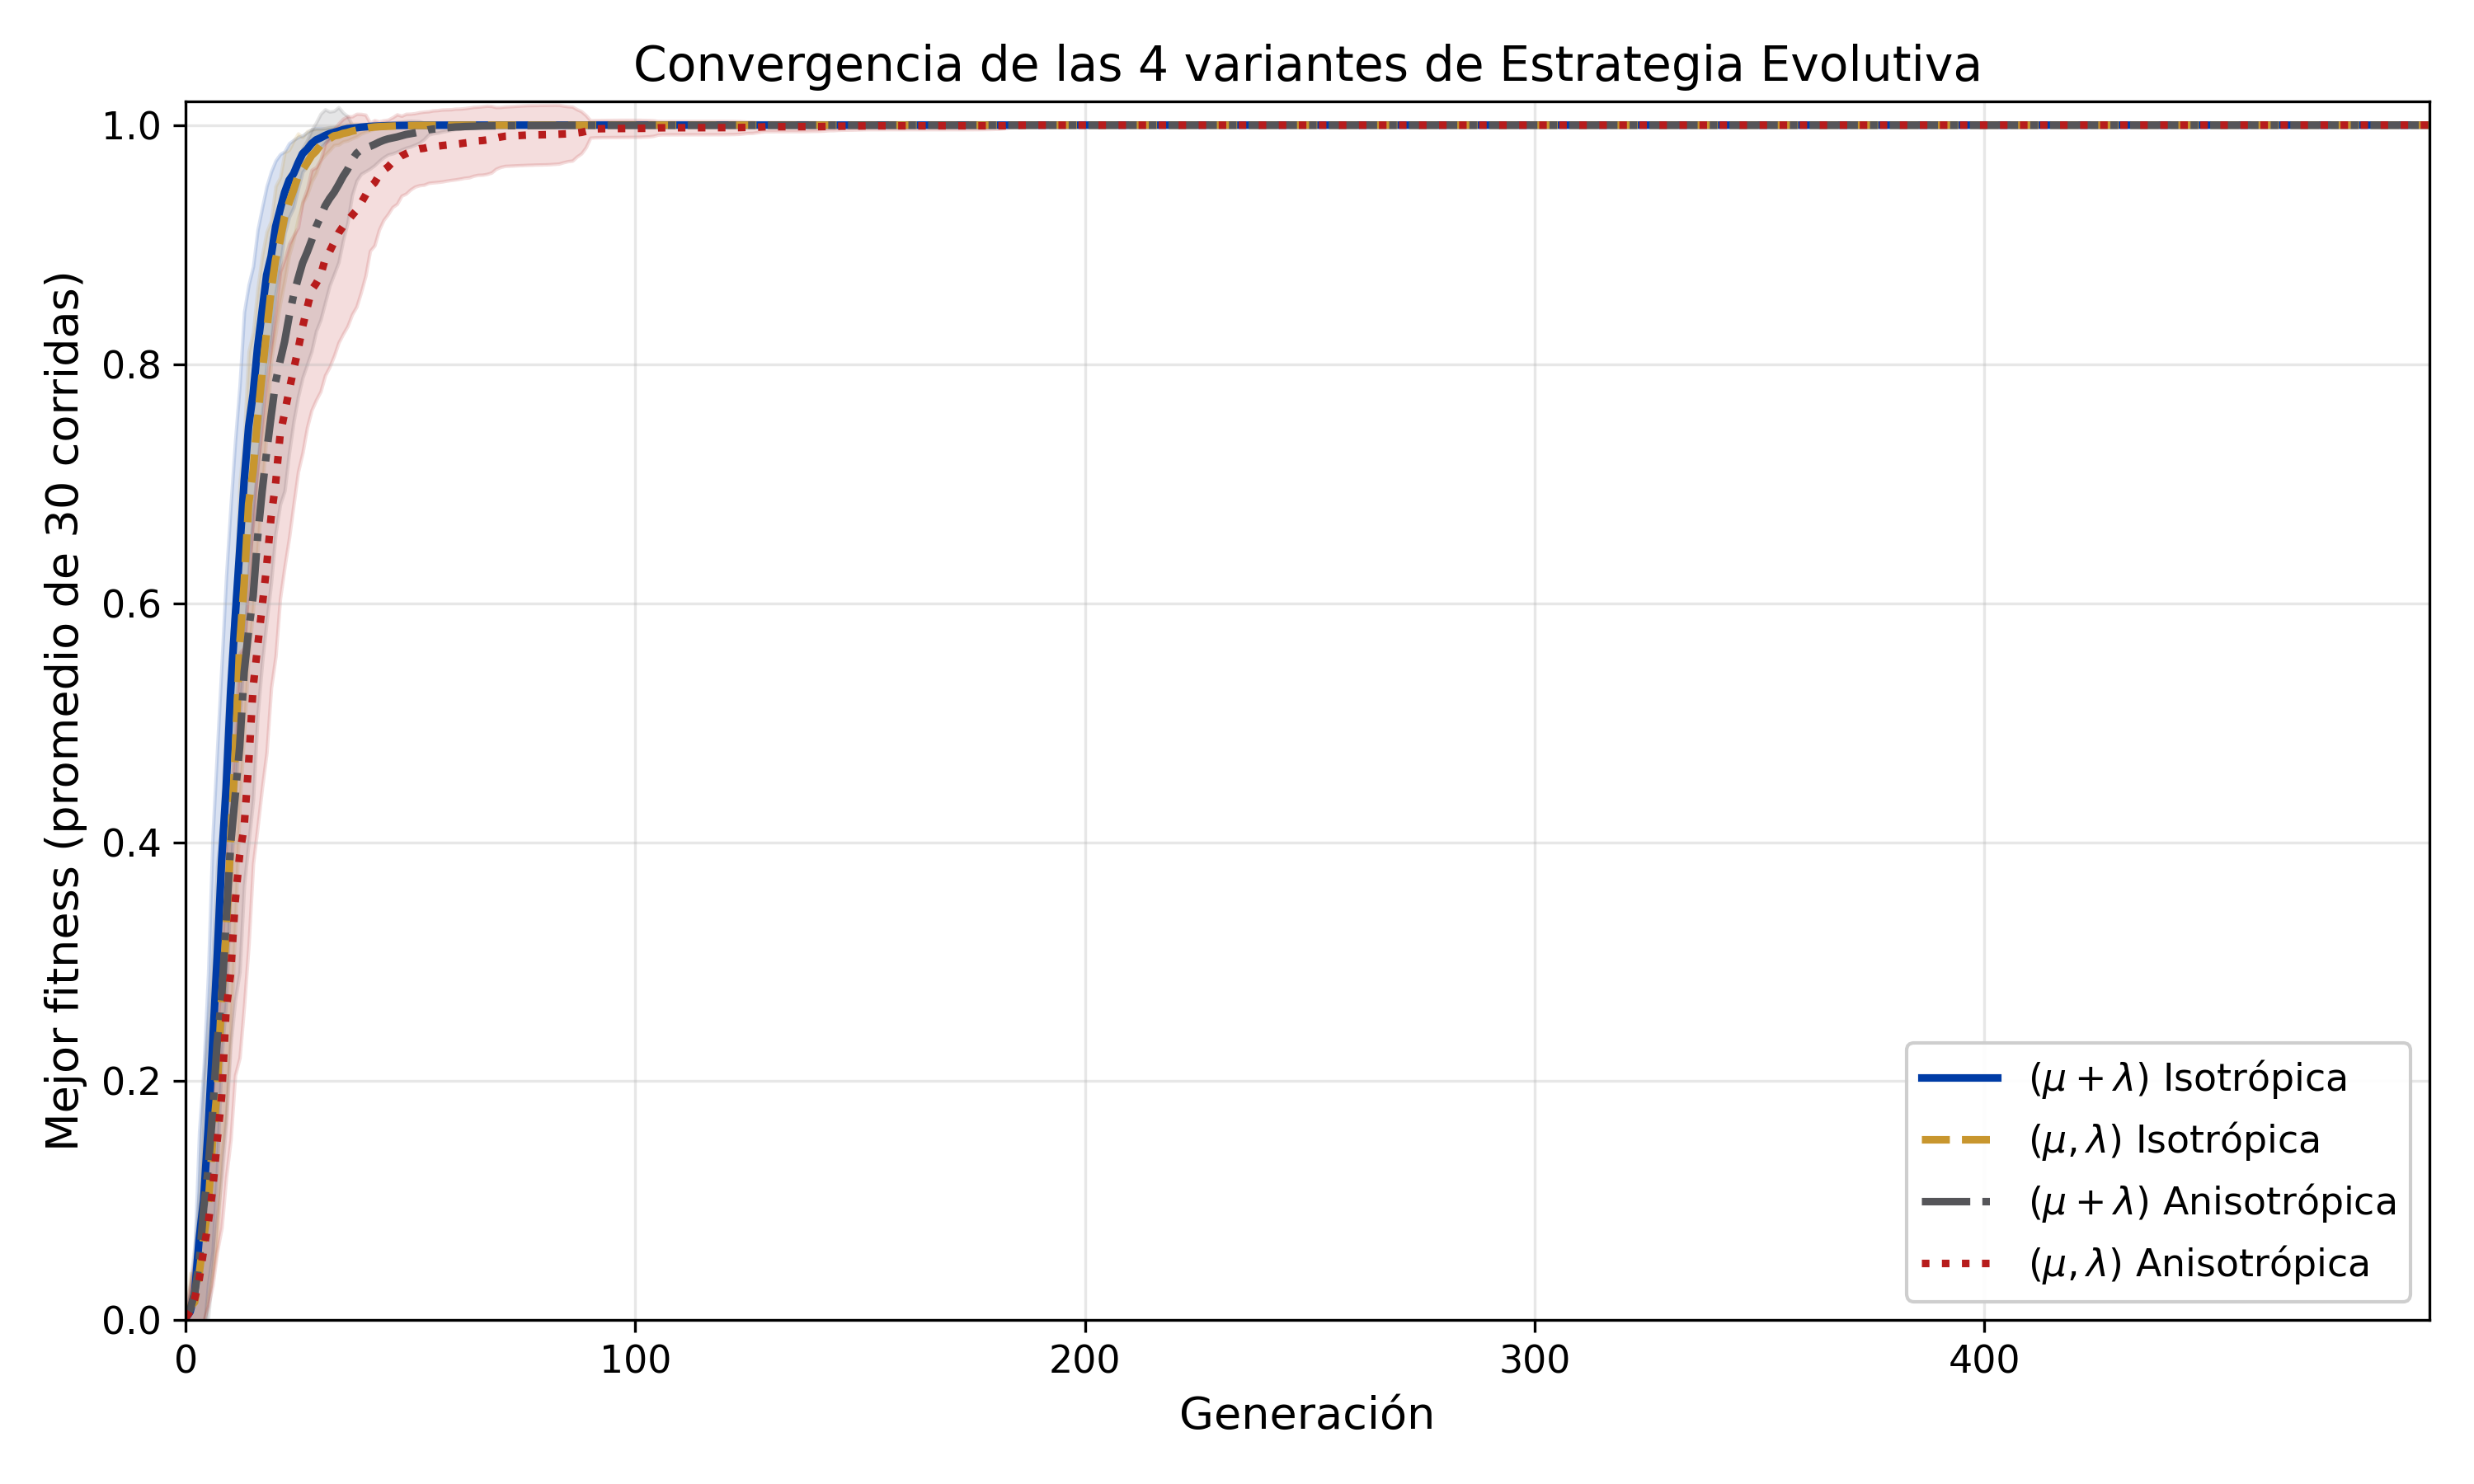
\includegraphics[width=\textwidth]{convergence_comparison.png}
    \caption[Convergencia promedio de las 4 variantes]{Convergencia del mejor fitness promediado en 30 corridas. Banda sombreada: $\pm 1$ desviación típica.}
    \label{fig:convergencia}
\end{figure}

La Figura~\ref{fig:convergencia_log} traslada el gráfico anterior a escala logarítmica del Gap~$1-f$, poniendo en evidencia la diferencia de velocidad de las variantes.

\begin{figure}[H]
    \centering
    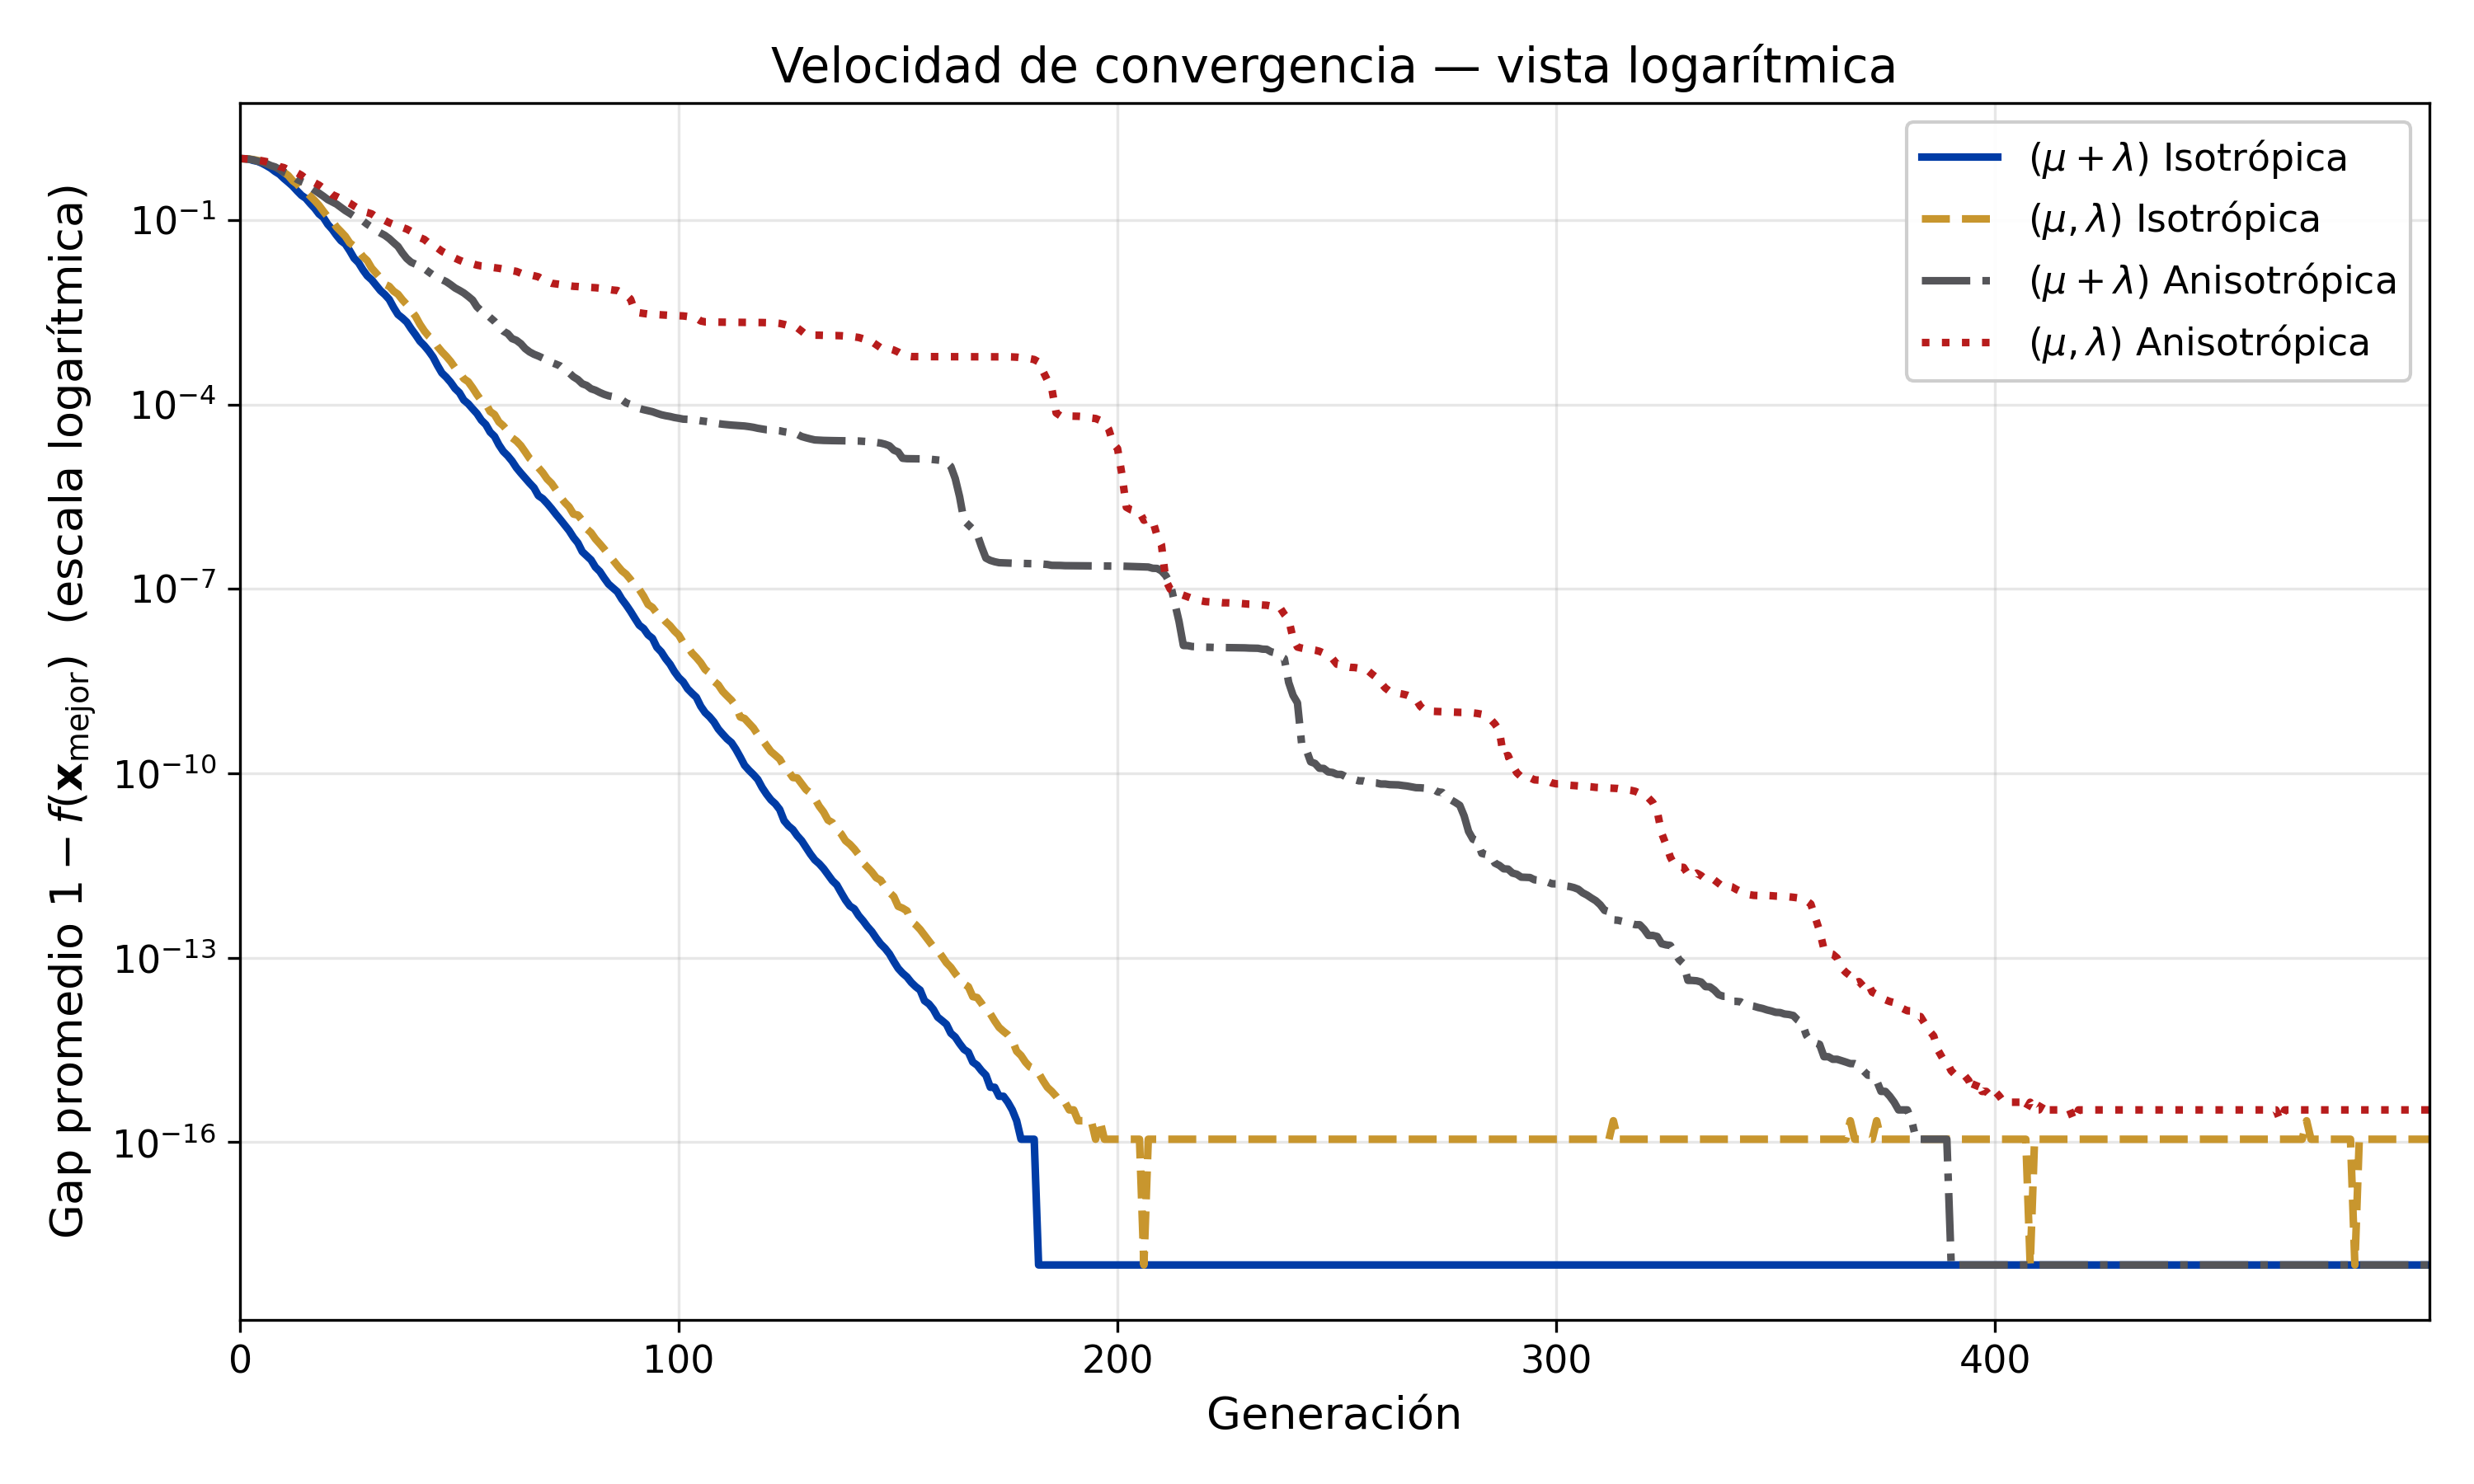
\includegraphics[width=\textwidth]{convergence_log.png}
    \caption[Convergencia en escala log del Gap]{Decaimiento del Gap promedio en escala logarítmica. La pendiente de cada curva indica la velocidad de progreso hacia el óptimo.}
    \label{fig:convergencia_log}
\end{figure}

\subsection{Tabla comparativa de desempeño}

La Tabla~\ref{tab:resultados} consolida los tres indicadores obligatorios de la rúbrica por variante: \textbf{Gap final} (media y desviación estándar sobre las 30 corridas), \textbf{Tasa de éxito} (porcentaje de corridas que alcanzan $f\geq 0.95$) y \textbf{velocidad de convergencia}. Como todas las corridas alcanzan el óptimo, el Gap final es numéricamente nulo y la tasa de éxito es del 100\,\%; el diferenciador es la velocidad de convergencia.

\begin{table}[H]
\centering
\caption[Resultados por variante]{Resultados agregados de las 30 corridas por variante. \textit{Gen}$\to$0.95: generación en la que el mejor fitness cruza el umbral por primera vez.}
\label{tab:resultados}
% VALORES GENERADOS DESDE results/per_variant_summary.json y results/summary.csv
\renewcommand{\arraystretch}{1.35}
\begin{tabular}{lcccc}
    \toprule
    \rowcolor{tablehead}
    \textcolor{white}{\textbf{Variante}} &
    \textcolor{white}{\textbf{Gap final (media $\pm\sigma$)}} &
    \textcolor{white}{\textbf{Éxito (\%)}} &
    \textcolor{white}{\textbf{Gen}$\bm{\to 0.95}$} &
    \textcolor{white}{\textbf{Mejor fitness prom.}} \\
    \midrule
    $(\mu+\lambda)$ Isotrópica    & $0 \pm 0$                                      & $100.0$ & $22.23 \pm  3.46$ & $1.000000$ \\
    \rowcolor{gray!8}
    $(\mu,\lambda)$ Isotrópica    & $1.74\times10^{-16} \pm 6.31\times10^{-17}$    & $100.0$ & $24.00 \pm  3.01$ & $1.000000$ \\
    $(\mu+\lambda)$ Anisotrópica  & $0 \pm 0$                                      & $100.0$ & $31.70 \pm  7.27$ & $1.000000$ \\
    \rowcolor{gray!8}
    $(\mu,\lambda)$ Anisotrópica  & $2.96\times10^{-16} \pm 1.02\times10^{-16}$    & $100.0$ & $39.23 \pm 13.78$ & $1.000000$ \\
    \bottomrule
\end{tabular}
\end{table}

\subsection{Velocidad al umbral de éxito}

La Figura~\ref{fig:gensucc} presenta la distribución (boxplot) del número de generaciones necesarias para cruzar $f\geq 0.95$. Cada variante anisotrópica es claramente más lenta y además más \textit{variable} (caja más alta) que su análoga isotrópica.

\begin{figure}[H]
    \centering
    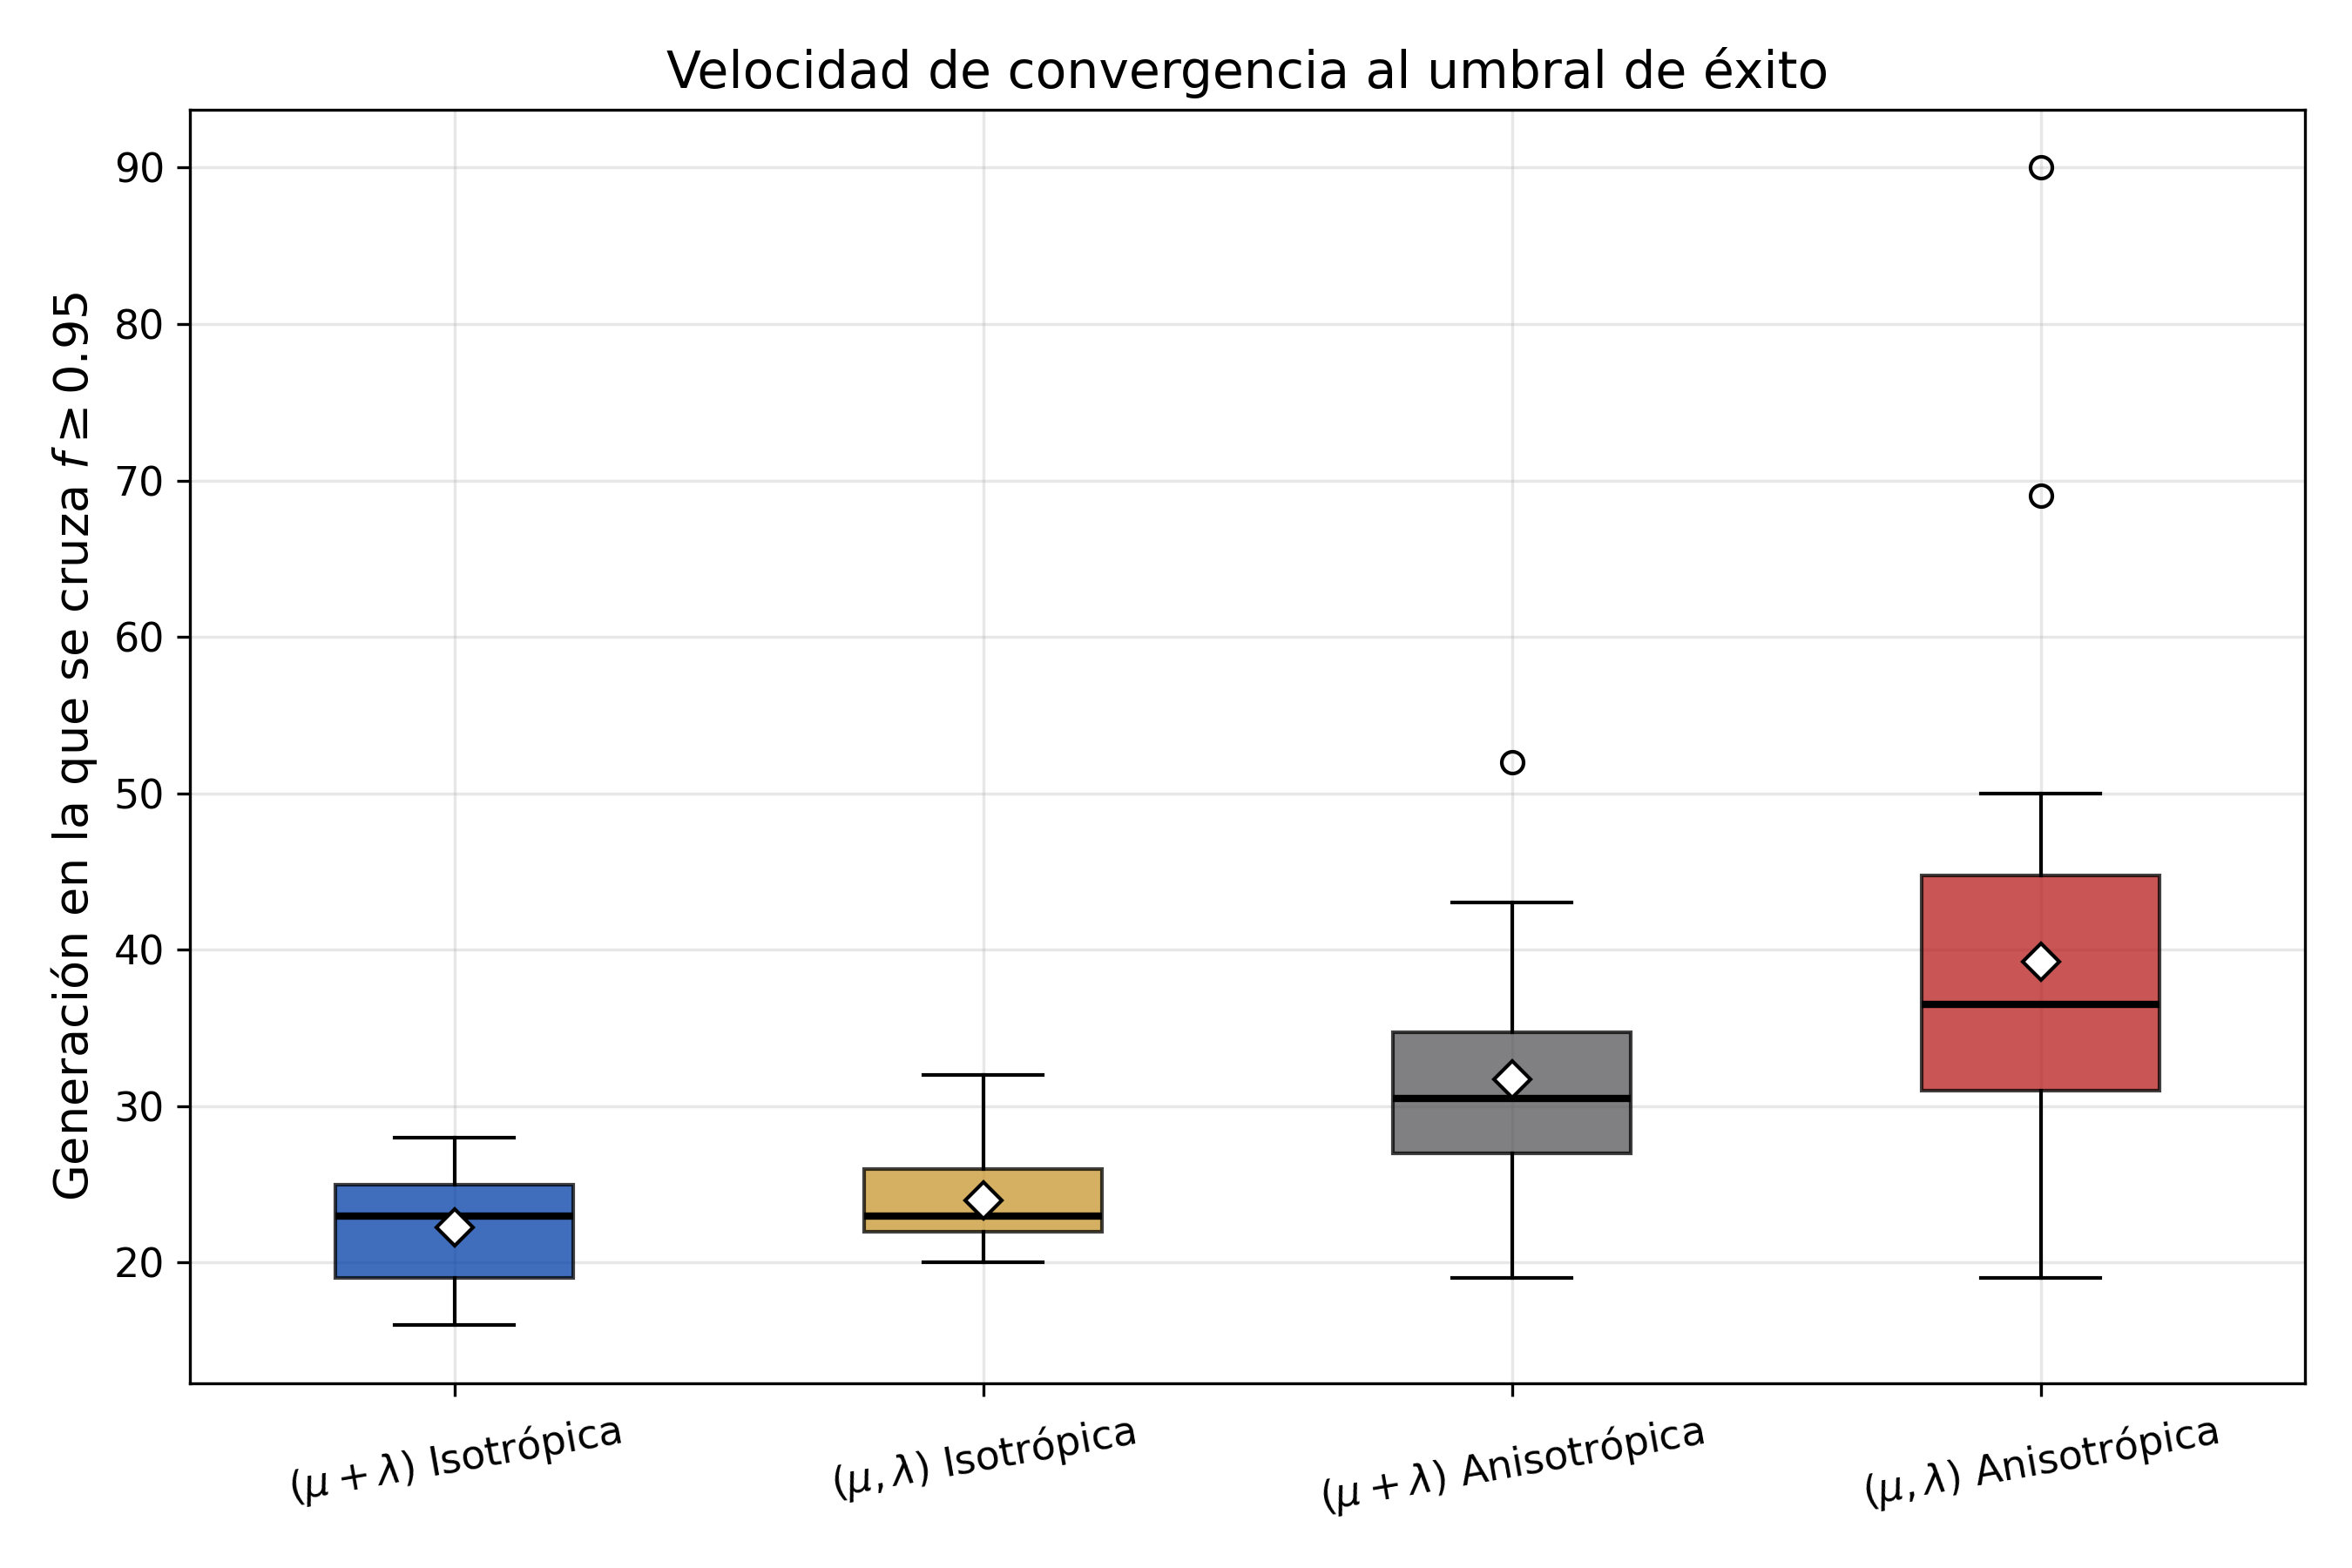
\includegraphics[width=0.85\textwidth]{generations_to_success.png}
    \caption[Distribución del número de generaciones hasta $f\geq 0.95$]{Boxplot con mediana, cuartiles y media (diamante) del número de generaciones necesarias para alcanzar el umbral de éxito.}
    \label{fig:gensucc}
\end{figure}

\subsection{Tasa de éxito y Gap}

Como soporte visual complementario, la Figura~\ref{fig:success} reporta la tasa de éxito (idéntica al 100\,\% en las cuatro variantes) y la Figura~\ref{fig:gap} el Gap final en escala logarítmica, evidenciando que las variantes \emph{coma} se quedan en la precisión numérica de doble precisión por no preservar padres.

\begin{figure}[H]
    \centering
    \begin{minipage}{0.48\textwidth}
        \centering
        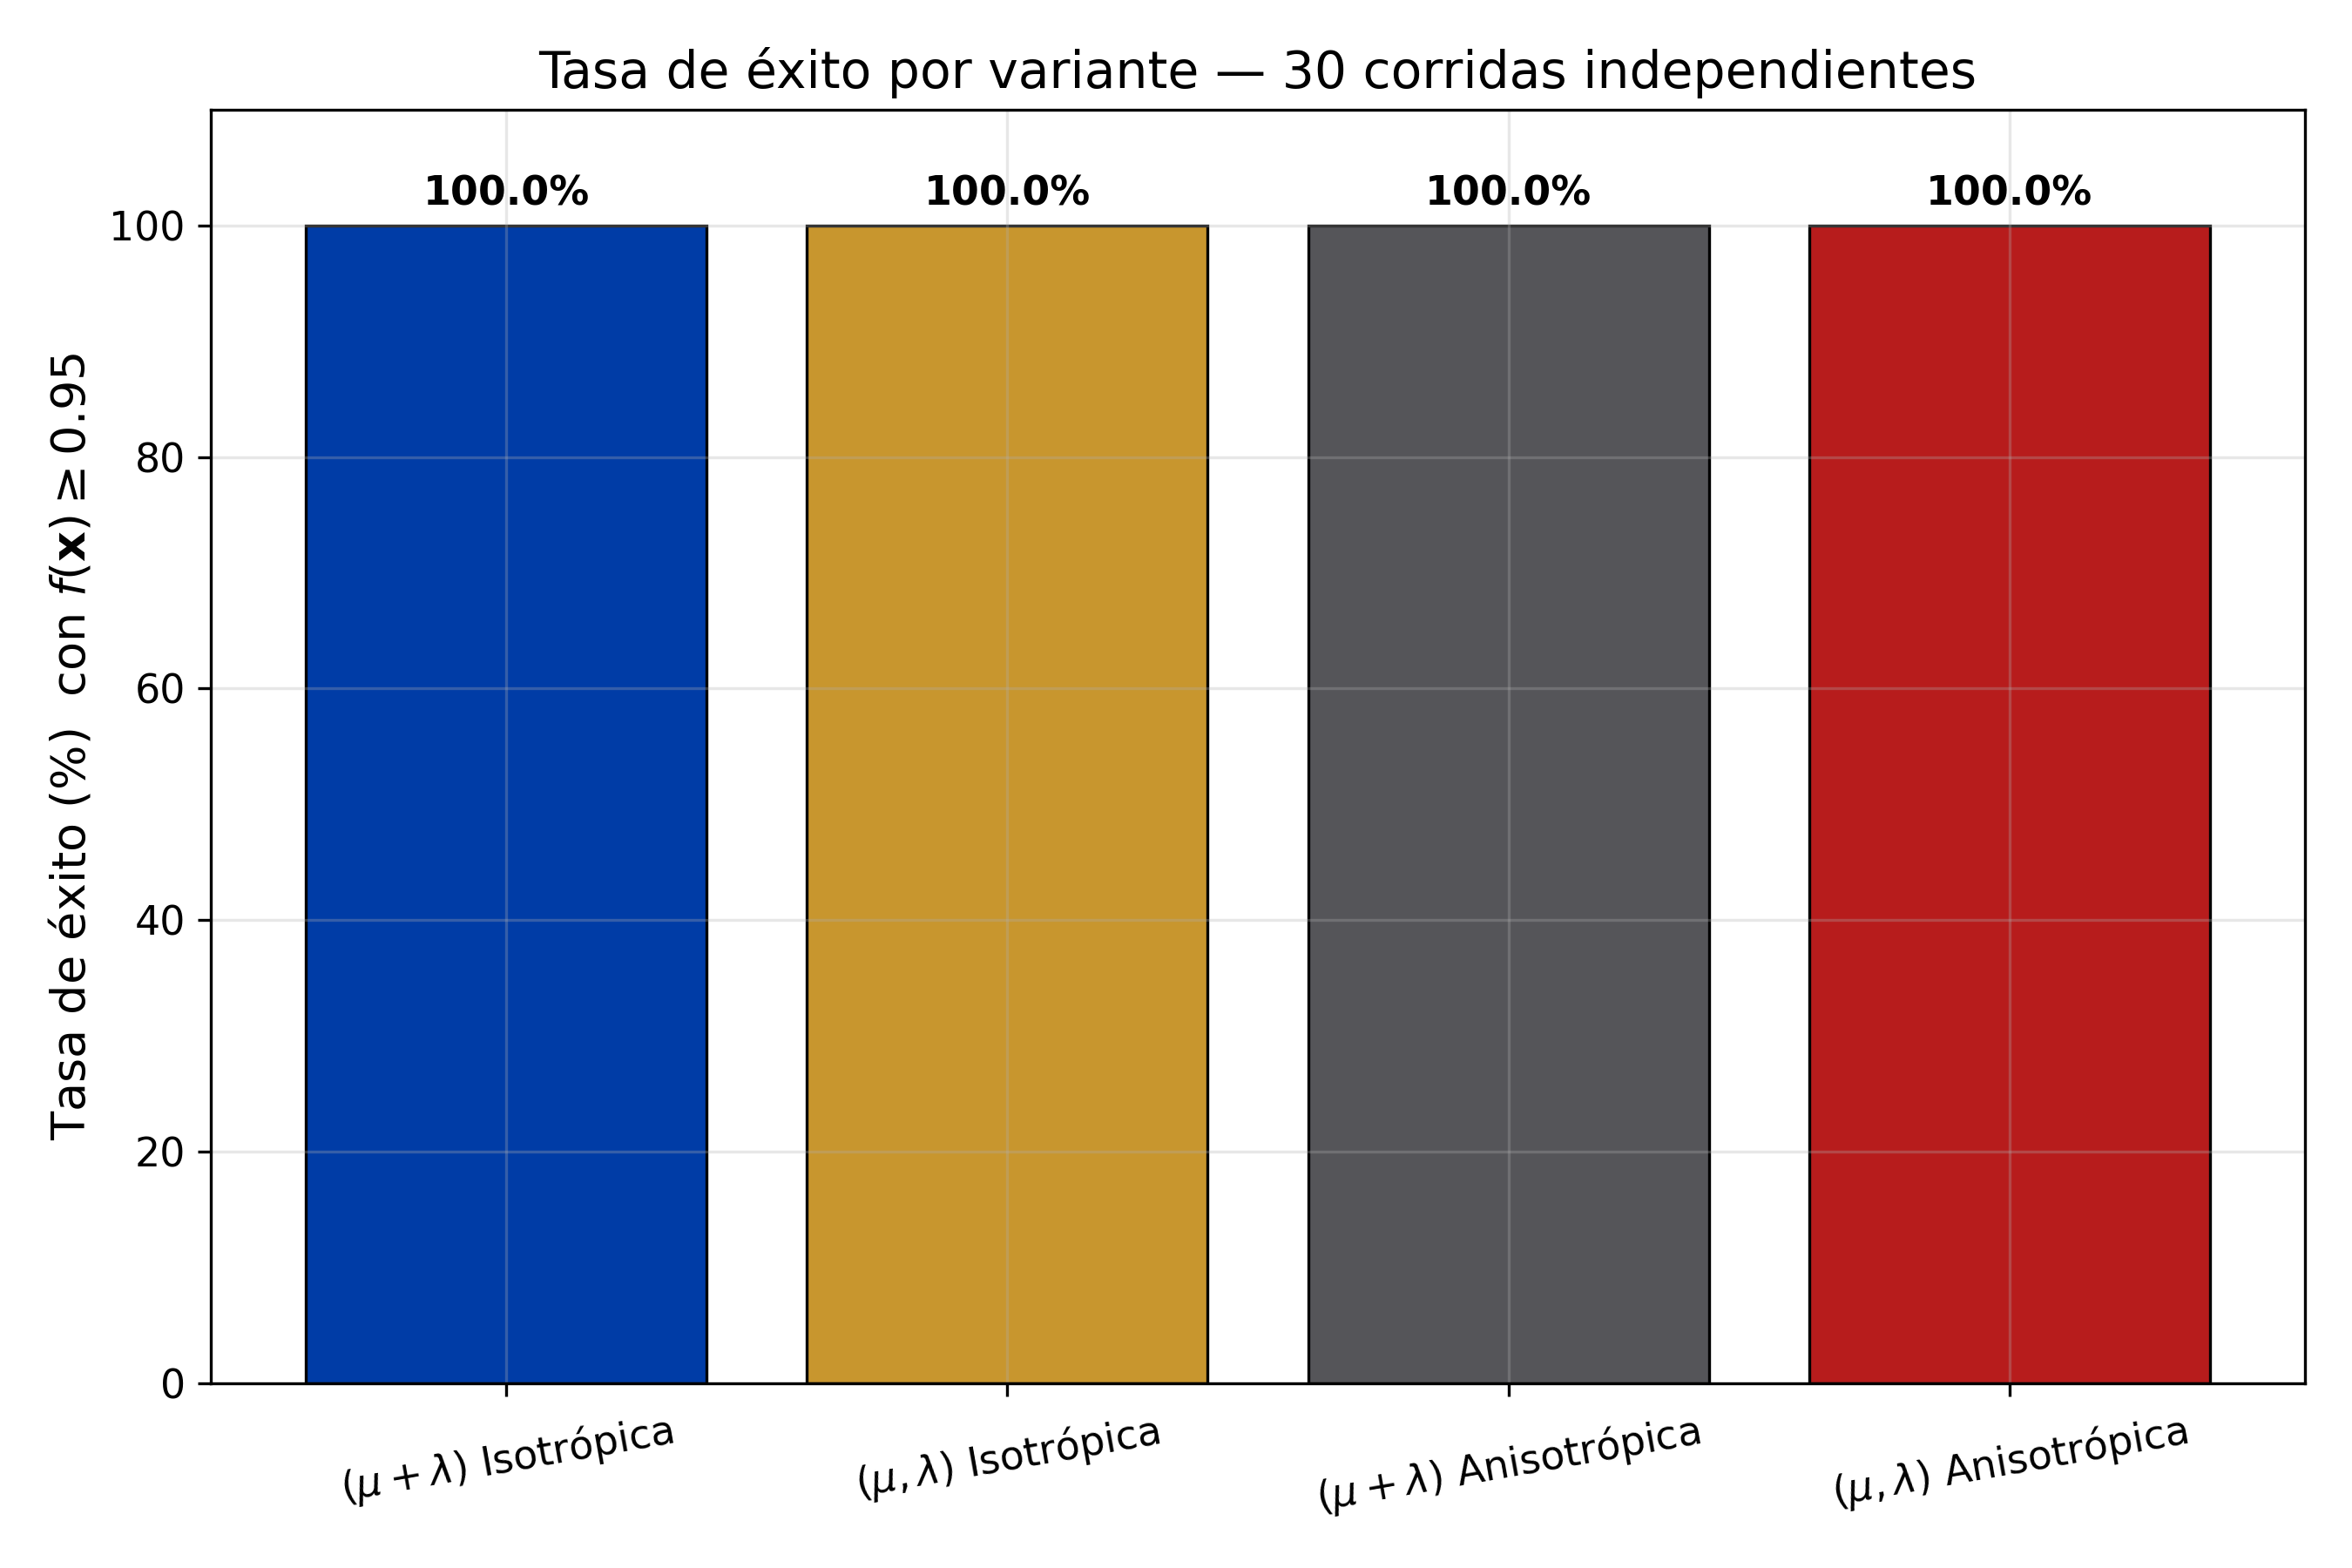
\includegraphics[width=\textwidth]{success_rate.png}
    \end{minipage}%
    \hfill
    \begin{minipage}{0.48\textwidth}
        \centering
        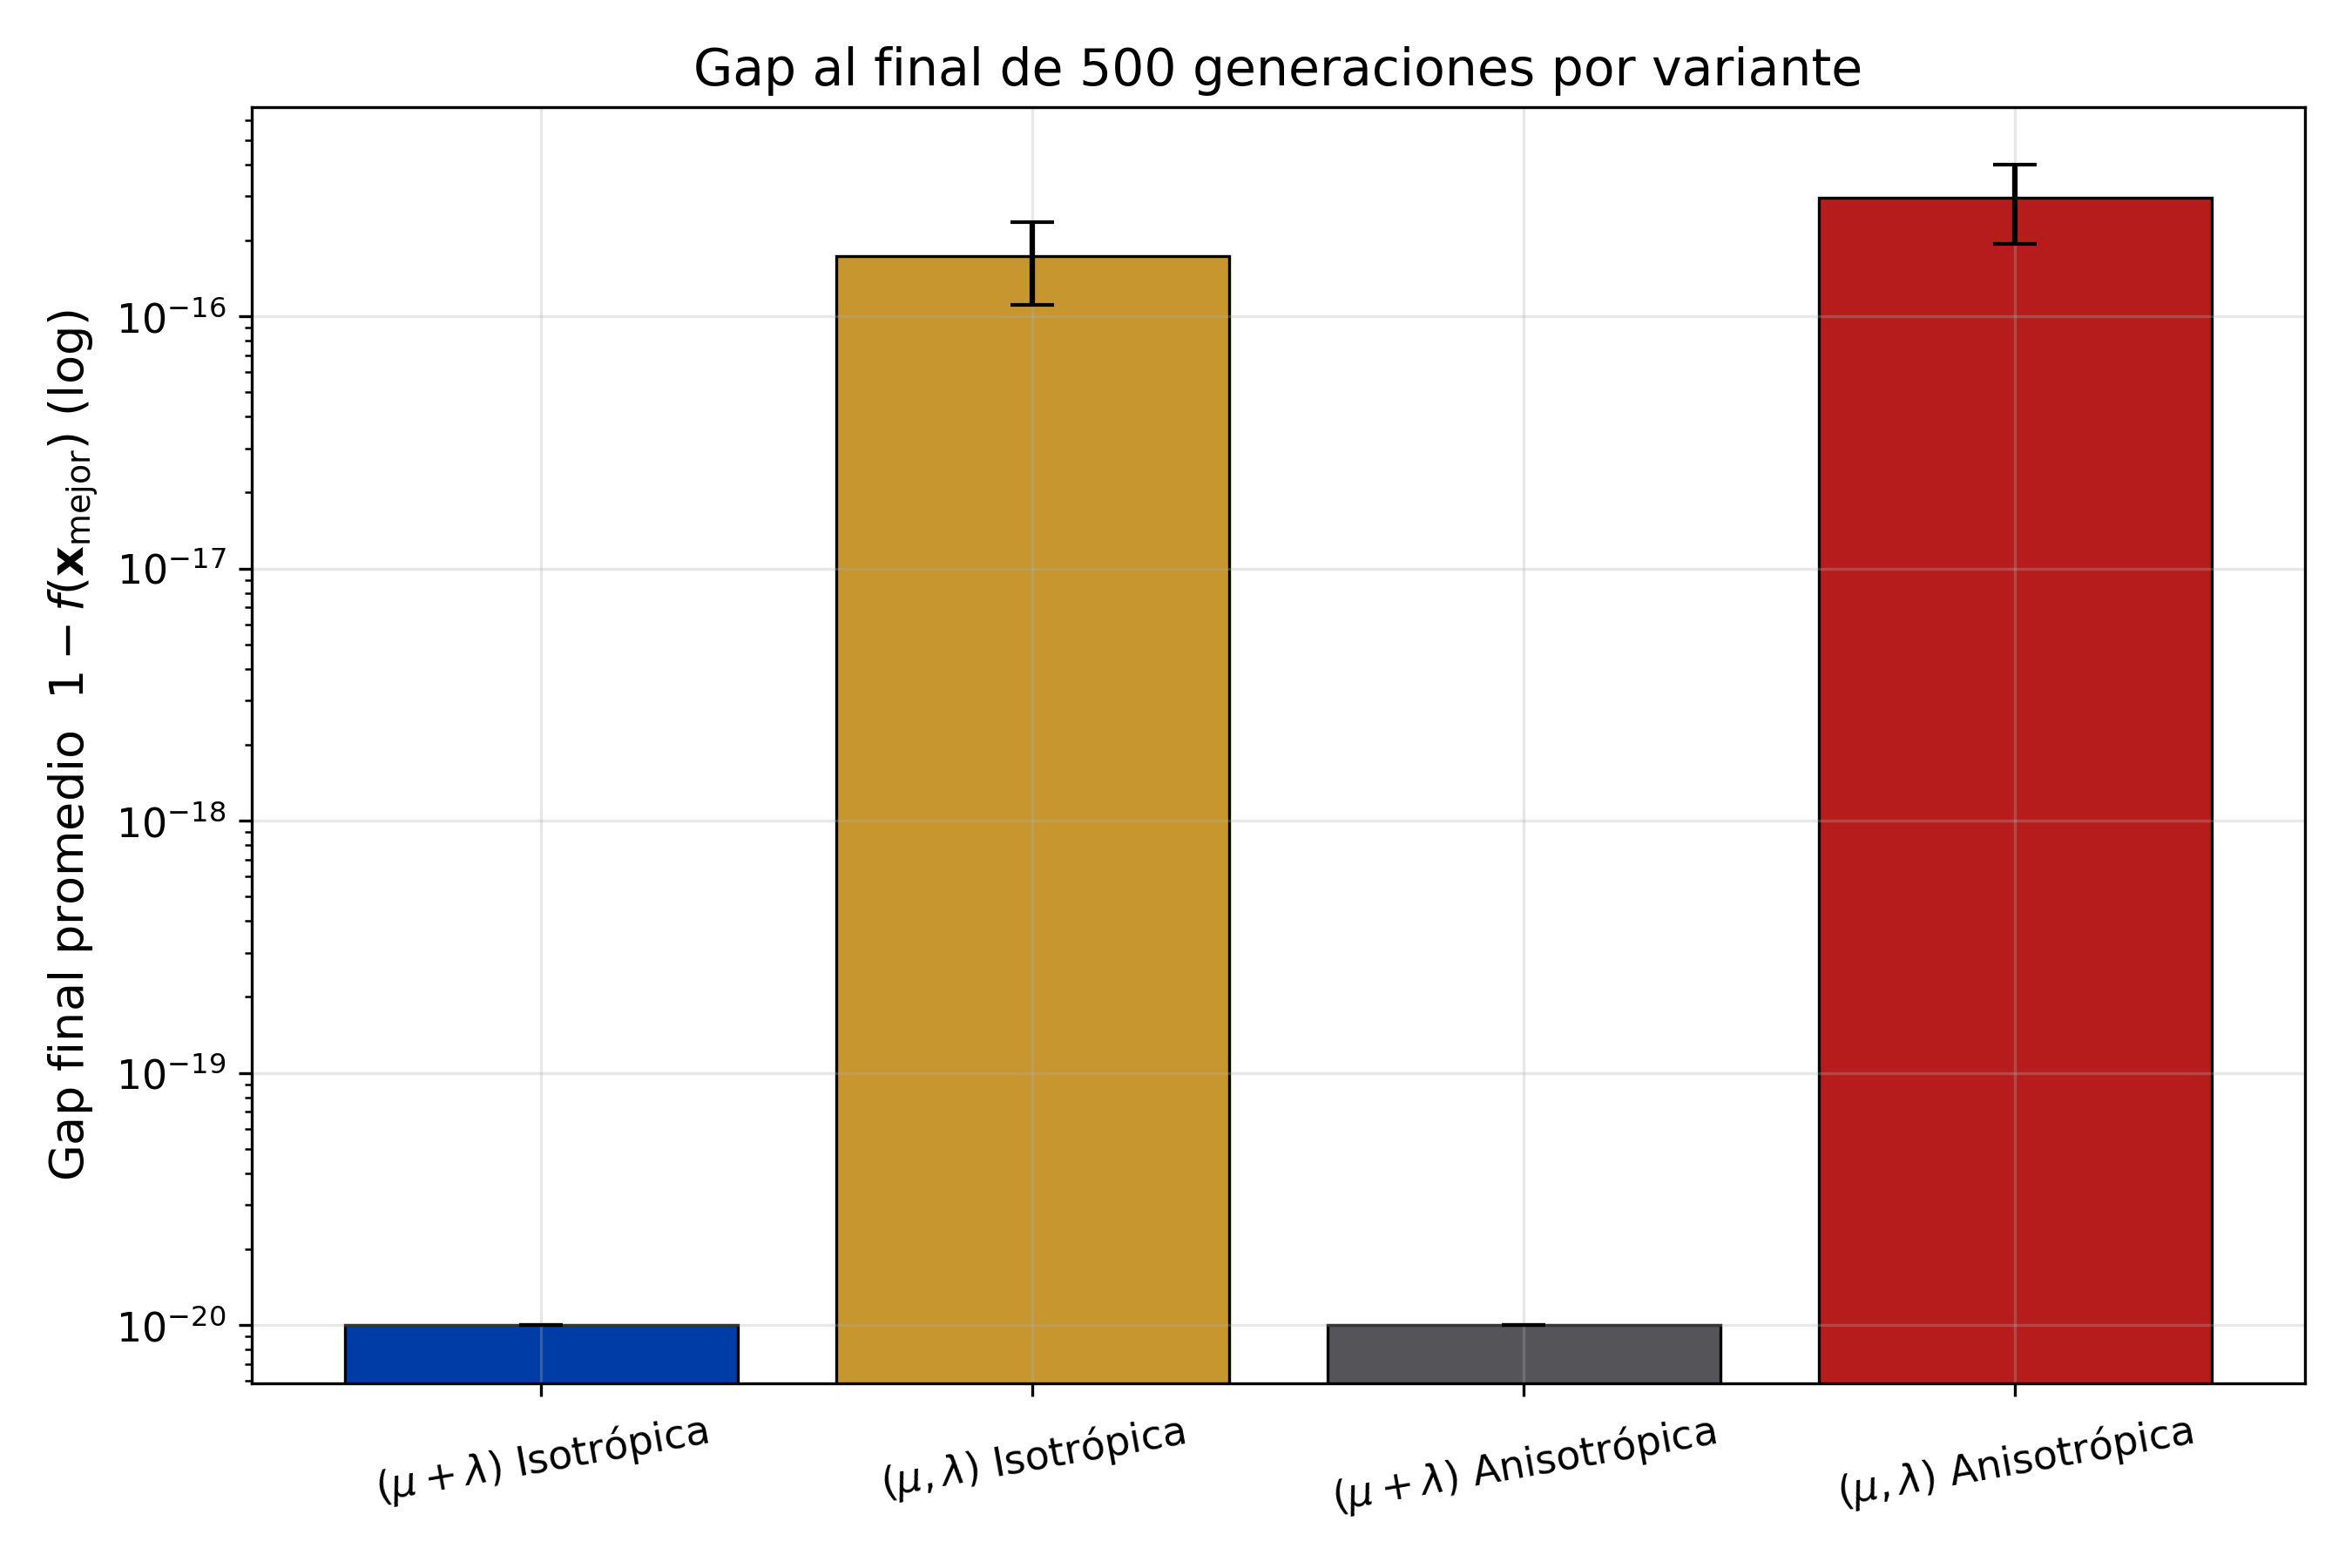
\includegraphics[width=\textwidth]{gap_comparison.png}
    \end{minipage}
    \caption[Tasa de éxito y Gap final por variante]{\textit{Izquierda:} tasa de éxito $f\geq 0.95$ (100\,\% en las cuatro variantes). \textit{Derecha:} Gap final en escala logarítmica; los esquemas $(\mu,\lambda)$ quedan limitados por el \textit{floor} numérico de la doble precisión.}
    \label{fig:success}\label{fig:gap}
\end{figure}

\subsection{Auto-adaptación de \texorpdfstring{$\sigma$}{sigma}}

La Figura~\ref{fig:sigma} es la evidencia directa del mecanismo de auto-adaptación. El panel izquierdo muestra el decaimiento exponencial del $\sigma$ único (isotrópico) a medida que la búsqueda se acerca al óptimo. El panel derecho ilustra el comportamiento clave de la anisotrópica: los $\sigma_i$ se separan y se ordenan por dimensión.

\begin{figure}[H]
    \centering
    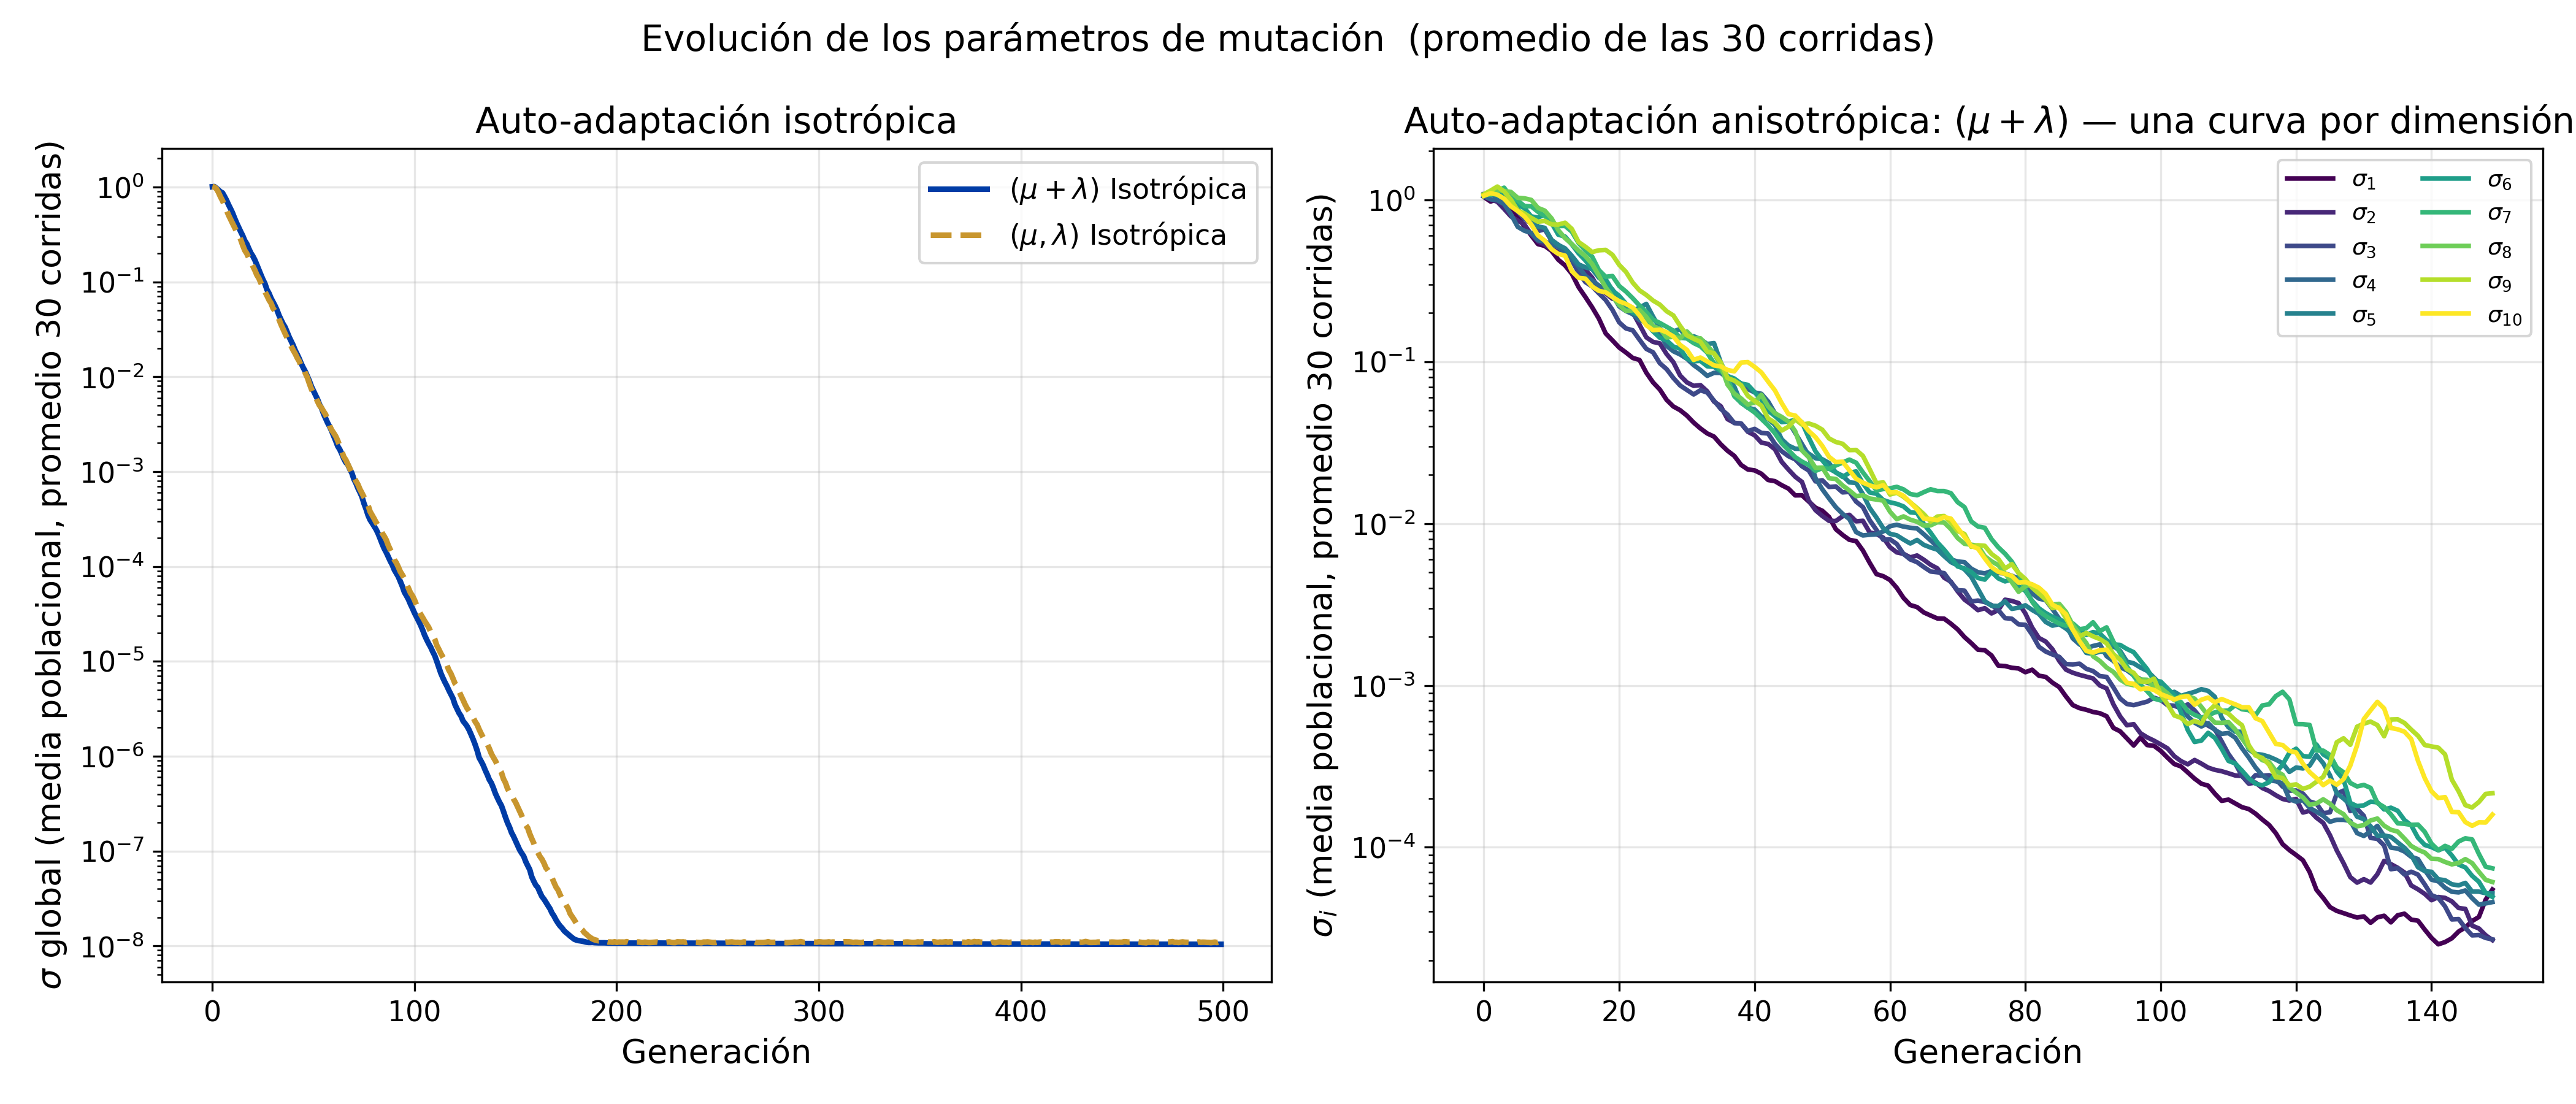
\includegraphics[width=\textwidth]{sigma_evolution.png}
    \caption[Evolución de los parámetros de mutación]{Evolución de los parámetros de mutación. \textbf{Izq.}: $\sigma$ global isotrópico (media poblacional, promediada en 30 corridas). \textbf{Der.}: los diez $\sigma_i$ de la anisotrópica. Nótese cómo $\sigma_1$ (dimensión más empinada) queda por debajo de $\sigma_{10}$ (dimensión más plana), tal como predice la teoría.}
    \label{fig:sigma}
\end{figure}

\begin{resultbox}
\textbf{Lectura cualitativa de la Figura~\ref{fig:sigma} (panel derecho):} alrededor de la generación~40, la media poblacional cumple $\sigma_{10}/\sigma_{1}\approx 4$, con las dimensiones intermedias ordenadas monótonamente. Esto confirma que el algoritmo \emph{aprende} la escala apropiada para cada coordenada, en línea con la predicción teórica $\sigma_i^{*}\propto\sqrt{i}$.
\end{resultbox}

\newpage
% ==========================================================
\section{Discusión}

\subsection{\texorpdfstring{¿Por qué la isotrópica es más rápida aquí?}{Por que la isotropica es mas rapida aqui?}}

La hipótesis inicial anticipaba que la anisotrópica dominaría gracias a su capacidad de ajustar un $\sigma$ por coordenada. Los datos matizan esta expectativa: en este problema la anisotrópica es \emph{más lenta} (tabla~\ref{tab:resultados}, $\approx 32$ generaciones frente a $\approx 22$ de la isotrópica).

La explicación es económica. El factor de auto-adaptación de la isotrópica tiene una varianza efectiva de $\tau^{2}=1/(2D)$ sobre \emph{un} parámetro escalar, mientras que la anisotrópica debe estabilizar $D=10$ parámetros con tasas $\tau_0^{2}+\tau_i^{2}$. Aunque la velocidad \emph{asintótica} de la anisotrópica podría ser superior si el número de condición del paisaje fuese extremo, en este caso el rango de pendientes cubre apenas un factor~$10$ (la relación entre denominadores $1$ y $10$). Con tan poca anisotropía, un único $\sigma$ global alcanza rápidamente un compromiso operativo ``lo bastante bueno'' para avanzar por todas las dimensiones, y la anisotrópica paga el coste de adaptar diez parámetros sin obtener una recompensa proporcional.

\subsection{\texorpdfstring{$(\mu+\lambda)$ vs $(\mu,\lambda)$}{(mu+lambda) vs (mu,lambda)}}

En ambas familias (iso y aniso), el esquema elitista $(\mu+\lambda)$ converge más rápido que $(\mu,\lambda)$ y alcanza un Gap final rigurosamente cero, mientras que $(\mu,\lambda)$ se queda en el \textit{floor} numérico de la doble precisión ($\sim 10^{-16}$). Esto es \emph{estructural}: al no preservar padres, $(\mu,\lambda)$ puede perder la mejor solución encontrada, y por eso fluctúa al nivel del ruido aritmético. En un paisaje multimodal, la misma propiedad sería una ventaja (permite escapar de óptimos locales), pero en un paisaje convexo como el elipsoide invertido solo añade varianza.

\subsection{\texorpdfstring{Evidencia del mecanismo de auto-adaptación}{Evidencia del mecanismo de auto-adaptacion}}

Aunque la anisotrópica \emph{pierde} en velocidad en este problema, su mecanismo se comporta como predice la teoría (Figura~\ref{fig:sigma}): los $\sigma_i$ se separan, las dimensiones empinadas ($i=1,2,3$) reciben un paso menor y las dimensiones planas ($i=8,9,10$) un paso mayor, con la relación cualitativa $\sigma_i\propto\sqrt{i}$. El algoritmo \emph{aprende} la escala adecuada sin que ninguna información sobre la función se le provea explícitamente: es la presión selectiva la que promueve las $\sigma_i$ útiles~\cite{beyer2001}.

\subsection{\texorpdfstring{Limitaciones del experimento}{Limitaciones del experimento}}

\begin{itemize}[leftmargin=2.2em, itemsep=3pt]
    \item \textbf{Problema de baja dimensión.} Con $D=10$ y número de condición $\kappa\approx 10$, la ventaja teórica de la anisotrópica es sutil. Repetir el experimento con $D=50$ y denominadores $i^{2}$ probablemente invertiría el ranking.
    \item \textbf{Sin recombinación.} La variante $\rho=1$ (un padre por descendiente) excluye la recombinación intermedia, que estabiliza los $\sigma_i$ y suele acelerar la auto-adaptación anisotrópica~\cite{eiben2015}.
    \item \textbf{$\sigma$ inicial único.} Inicializar $\sigma_0=1$ para todas las dimensiones introduce un sesgo contra la anisotrópica, que debe ``aprender'' partiendo de cero la escala por coordenada.
    \item \textbf{Criterio de éxito.} El umbral $f\geq 0.95$ es generoso; con umbrales más estrictos (por ejemplo $f\geq 1 - 10^{-6}$) la comparación entre los esquemas $(\mu+\lambda)$ y $(\mu,\lambda)$ se vuelve más severa.
\end{itemize}

\newpage
% ==========================================================
\section{Conclusiones}

% --- Foto + párrafo introductorio lado a lado ---
\noindent
\begin{minipage}[t]{3.6cm}
    \vspace{0pt}
    \centering
    
\includegraphics[width=3.3cm, height=3.3cm, keepaspectratio]{javiprofile.jpg}
\end{minipage}%
\hfill
\begin{minipage}[t]{\dimexpr\textwidth-4.2cm\relax}
    \vspace{0pt}
    Esta práctica deja una lección concreta: la sofisticación aparente de un mecanismo --en este caso la auto-adaptación anisotrópica-- no garantiza mejor desempeño; su beneficio depende de la topología del problema. El experimento con 120~ejecuciones confirma que las cuatro variantes encuentran el óptimo, pero revela diferencias de velocidad y estabilidad que no son visibles en las métricas de cierre.
\end{minipage}

\medskip

\begin{enumerate}[leftmargin=2.2em, itemsep=4pt]
    \item \textbf{Todas las variantes resuelven el problema.} Con $\mu=20$, $\lambda=100$ y 500 generaciones, la tasa de éxito es del 100\,\% en las cuatro variantes y el Gap final es numéricamente nulo.
    \item \textbf{El esquema $(\mu+\lambda)$ domina en velocidad y estabilidad.} El elitismo evita perder la mejor solución y elimina fluctuaciones al nivel del ruido aritmético de la doble precisión. En un paisaje unimodal la no-elitista no aporta valor.
    \item \textbf{La mutación isotrópica fue más rápida que la anisotrópica en este paisaje.} El número de condición $\kappa\approx 10$ es demasiado moderado para que los 10 parámetros anisotrópicos ganen a un único $\sigma$ bien ajustado. La teoría de Schwefel se verifica, pero el beneficio del vector $\boldsymbol{\sigma}$ se paga con generaciones extra de adaptación.
    \item \textbf{La auto-adaptación se observa directamente.} El panel derecho de la Figura~\ref{fig:sigma} muestra que los $\sigma_i$ se separan y se ordenan según la pendiente local del paisaje, con una relación cualitativa $\sigma_i\propto\sqrt{i}$, exactamente como predice la teoría.
    \item \textbf{Analogía con gestión bancaria de riesgo.} La elección entre isotropía y anisotropía guarda paralelo con la calibración de tolerancia al riesgo: aplicar un umbral uniforme a todos los productos (isotropía) es rápido y robusto cuando las carteras son homogéneas; diferenciar el umbral por producto (anisotropía) mejora la asignación cuando los riesgos difieren sustancialmente, pero exige datos e inversión para estimar cada parámetro. La misma lección observada en este experimento aplica en el día a día en Santander: sofisticar siempre cuesta, y la ganancia depende de la heterogeneidad real del problema.
\end{enumerate}

\vspace{1em}
{\color{uacjgray}\hrule}
\vspace{1em}

\newpage
% ==========================================================
% REFERENCIAS — formato IEEE, columna doble
% ==========================================================
\section*{Referencias}
\addcontentsline{toc}{section}{Referencias}

\begingroup
\renewcommand{\section}[2]{}
\begin{multicols}{2}
\small
\emergencystretch=3em
\begin{thebibliography}{10}

\bibitem{rechenberg1973}
I.~Rechenberg, \textit{Evolutionsstrategie: Optimierung technischer Systeme nach Prinzipien der biologischen Evolution}. Stuttgart, Alemania: Frommann-Holzboog, 1973.

\bibitem{schwefel1995}
H.-P. Schwefel, \textit{Evolution and Optimum Seeking}. New York, NY, USA: Wiley, 1995.

\bibitem{beyer2002}
H.-G. Beyer and H.-P. Schwefel, ``Evolution Strategies --- A Comprehensive Introduction,'' \textit{Natural Computing}, vol.~1, no.~1, pp.~3--52, 2002. doi:~10.1023/A:1015059928466.

\bibitem{beyer1995}
H.-G. Beyer, ``Toward a Theory of Evolution Strategies: Self-Adaptation,'' \textit{Evolutionary Computation}, vol.~3, no.~3, pp.~311--347, 1995.

\bibitem{beyer2001}
H.-G. Beyer and K.~Deb, ``On Self-Adaptive Features in Real-Parameter Evolutionary Algorithms,'' \textit{IEEE Trans.\ on Evolutionary Computation}, vol.~5, no.~3, pp.~250--270, 2001.

\bibitem{eiben2015}
A.~E. Eiben and J.~E. Smith, \textit{Introduction to Evolutionary Computing}, 2nd~ed. Berlin, Alemania: Springer, 2015. doi:~10.1007/978-3-662-44874-8.

\bibitem{back1997}
T.~Bäck, U.~Hammel, and H.-P. Schwefel, ``Evolutionary Computation: Comments on the History and Current State,'' \textit{IEEE Trans.\ on Evolutionary Computation}, vol.~1, no.~1, pp.~3--17, 1997.

\bibitem{porras2026ee}
R.~G. Porras~Alaniz, ``Práctica de Estrategias Evolutivas: Isotropía vs Anisotropía,'' Actividad de clase, Maestría en IA y Analítica de Datos, Universidad Autónoma de Ciudad Juárez (UACJ), 2026.

\bibitem{porras2026ag}
R.~G. Porras~Alaniz, ``Programando un Algoritmo Genético desde Cero para el VRP,'' Actividad de clase, Maestría en IA y Analítica de Datos, UACJ, 2026.

\end{thebibliography}
\end{multicols}
\endgroup

\end{document}
